\newpage
	\section{Цель и задачи работы}
		\textbf{Цель работы}: приобретение практических навыков реализации важнейших элементов лексических анализаторовна
			примере распознавания цепочек регулярного языка.\\

		\textbf{Задачи работы:}
		\begin{enumerate}
			\item Ознакомиться с основными понятиями и определениями, лежащими в основе построения лексических анализаторов.
			\item Прояснить связь между регулярным множеством, регулярным выражением, праволинейным языком,
				конечно-автоматным языком и недетерминированным конечно-автоматным языком.
			\item Разработать, тестировать и отладить программу распознавания цепочек регулярного или
				праволинейного языка в соответствии с предложенным вариантом грамматики.
		\end{enumerate}


%%%%%%%%%%%%%%%%%%%%%%%%%%%%%%
	\section{Листинг}
        
        \lstset{inputencoding=utf8x, extendedchars=\true, breaklines=true, numbers=left,
        keywordstyle=\color{blue}, commentstyle=\color{red}}
        
        \subsection{main.py}
        \lstinputlisting[language=python]{../../main.py}

        \subsection{regexp\_process.py}
        \lstinputlisting[language=python]{../../regexp_process.py}

        \subsection{FSM.py}
        \lstinputlisting[language=python]{../../FSM.py}

        \subsection{utils.py}
        \lstinputlisting[language=python]{../../utils.py}

%%%%%%%%%%%%%%%%%%%%%%%%%%%%%%
	\section{Проверка корректности программы}
		Все тесты производятся для алфавита $\Sigma = \{a, b\}$, конкатенация заменяется на символ <<.>>,
		начальные состояния имеют в названии символ <<s>>, а финальные <<f>>.
		\subsubsection{Выражение $ab$}
			\textbf{Постфиксное регулярное выражение:}\\
				$ab.$

			\newpage
			\textbf{НКА:}
				\begin{figure}[h!]
					\begin{center}
						\includegraphics[scale=0.6]{ab/nka.png}
					\end{center}
				\end{figure}

			\textbf{ДКА:}
				\begin{figure}[h!]
					\begin{center}
						\includegraphics[scale=0.6]{ab/dka.png}
					\end{center}
				\end{figure}
			
			\newpage
			\textbf{Минимальный ДКА:}
				\begin{figure}[h!]
					\begin{center}
						\includegraphics[scale=0.6]{ab/dka_min.png}
					\end{center}
				\end{figure}

		
		\subsubsection{Выражение $a*$}
		\textbf{Постфиксное регулярное выражение:}\\
			$a*$

		\textbf{НКА:}
			\begin{figure}[h!]
				\begin{center}
					\includegraphics[scale=0.5]{a_star/nka.png}
				\end{center}
			\end{figure}

		\newpage
		\textbf{ДКА:}
			\begin{figure}[h!]
				\begin{center}
					\includegraphics[scale=0.6]{a_star/dka.png}
				\end{center}
			\end{figure}

		\textbf{Минимальный ДКА:}
			\begin{figure}[h!]
				\begin{center}
					\includegraphics[scale=0.6]{a_star/dka_min.png}
				\end{center}
			\end{figure}

		\subsubsection{Выражение $(a|b)*abb$}
		\textbf{Постфиксное регулярное выражение:}\\
			$ab|*a.b.b.$

		\newpage
		\textbf{НКА:}
			\begin{figure}[h!]
				\begin{center}
					\includegraphics[scale=0.5]{complex/nka.png}
				\end{center}
			\end{figure}

		\newpage
		\textbf{ДКА:}
			\begin{figure}[h!]
				\begin{center}
					\includegraphics[scale=0.6]{complex/dka.png}
				\end{center}
			\end{figure}

		\textbf{Минимальный ДКА:}
			\begin{figure}[h!]
				\begin{center}
					\includegraphics[scale=0.6]{complex/dka_min.png}
				\end{center}
			\end{figure}

%%%%%%%%%%%%%%%%%%%%%%%%%%%%%%

	\newpage
	\section{Выводы}
	
	По результатам проведенной работы студент ознакомился с основными определениями и понятиями, лежащими в основе
		построения лексических анализаторов и приобрел опыт в их реализации.
	В том числе была реализована программа, принимающая грамматику, по которой строится допускающий ее НКА, ДКА и минимальный ДКА, 
		а также моделируется работа минимального ДКА для проверки входной цепочки символов

%%%%%%%%%%%%%%%%%%%%%%%%%%%%%%

	\section{Список литературы}
		\begin{enumerate}
			\item БЕЛОУСОВ А.И., ТКАЧЕВ С.Б. Дискретная математика: Учеб. Для вузов / Под ред. В.С. Зарубина, А.П. Крищенко. – М.: Изд-во МГТУ им. Н.Э. Баумана, 2001.
			\item АХО А., УЛЬМАН Дж. Теория синтаксического анализа, перевода и компиляции: В 2-х томах. Т.1.: Синтаксичечкий анализ. - М.: Мир, 1978.
			\item АХО А.В, ЛАМ М.С., СЕТИ Р., УЛЬМАН Дж.Д. Компиляторы: принципы, технологии и инструменты. – М.: Вильямс, 2008.
		\end{enumerate}
	